% elementos pós-textuais 
\postextual

% apêndice 
\begin{apendicesenv}
\partapendices

% Apêndice A
\chapter{DEMONSTRAÇÕES} \label{apendice_demonstracoes}

% proposição 1
\begin{proposition}[condição de ausência de viés em $\mathbfit{\tilde{y}}$]
  \label{proposicao1}

  Se as previsões reconciliadas são não viesadas, então $\mathbfit{SGS=S}$, ou seja, $\mathbfit{G}$ é inversa generalizada de $\mathbfit{S}$.

\end{proposition}

\begin{proof}
  \begin{equation} \label{eq:ap1}
    \mathbfit{\tilde{y}}_{t+h|t} = \mathbfit{SG\hat{y}}_{t+h|t} 
  \end{equation}

  Se $\mathbfit{\hat{y}}_{t+h|t}$ é não viesado, então 

  \begin{equation} \label{eq:ap2}
      \mathbb{E}[\mathbfit{\hat{y}}_{t+h|t}] = \mathbb{E}[\mathbfit{y}_{t+h|t}] = \mathbfit{Sb}_t
  \end{equation}

  Da mesma forma, se espera-se que as previsões reconciliadas não sejam viesadas,
  \begin{equation} \label{eq:ap3}
      \mathbb{E}[\mathbfit{\tilde{y}}_{t+h|t}] = \mathbb{E}[\mathbfit{y}_{t+h|t}] = \mathbfit{Sb}_t
  \end{equation}

  Substituindo \eqref{eq:ap2} em \eqref{eq:ap1}, temos

  \begin{equation} \label{eq:ap4}
      \mathbfit{\tilde{y}}_{t+h|t} = \mathbfit{SGSb}_t 
  \end{equation}

  Logo, para manter a igualdade entre \eqref{eq:ap1} e \eqref{eq:ap4}, $\mathbfit{SGS=S}$

\end{proof}

% proposição 2
\begin{proposition}
  \label{proposicao2}

  $\mathbfit{\tilde{e}}_t = \mathbfit{SG\hat{e}}_t$.

\end{proposition}

\begin{proof}
  \begin{equation} \label{eq:apa22}
    \mathbfit{\tilde{e}}_{t+h|t} = \mathbfit{y}_{t+h} - \mathbfit{\tilde{y}}_{t +h|t}
  \end{equation}

  Substituindo \eqref{eq:ap1} em \eqref{eq:apa22},

  \begin{align} \label{eq:apa23}
    \mathbfit{\tilde{e}}_{t+h|t} &= \mathbfit{y}_{t+h} - \mathbfit{SG\hat{y}}_{t+h|t}
  \end{align}

  Lembrando que, por definição, $\mathbfit{y}_{t+h} = \mathbfit{\hat{y}}_{t+h|t} + \mathbfit{\hat{e}}_{t+h|t}$, então

  \begin{align} \label{eq:apa24}
    \mathbfit{\tilde{e}}_{t+h|t} &= \mathbfit{\hat{y}}_{t+h|t} + \mathbfit{\hat {e}}_{t+h|t} - \mathbfit{SG\hat{y}}_{t+h|t} \\
    &= \mathbfit{\hat{e}}_{t+h|t} + \mathbfit{\hat{y}}_{t+h|t}(\mathbfit{I-SG)}
  \end{align}

  Usando a definição novamente, temos que

  \begin{align}
    \mathbfit{\tilde{e}}_{t+h|t} &= \mathbfit{\hat{e}}_{t+h|t} + (\mathbfit{y}_ {t+h} - \mathbfit{\hat{e}}_{t+h|t})(\mathbfit{I-SG)} \\
    &= \mathbfit{y}_{t+h} - \mathbfit{SGy}_{t+h|t} + \mathbfit{SG\hat{e}}_{t+h| t} \\
    &=  \mathbfit{y}_{t+h}(\mathbfit{I-SG}) + \mathbfit{SG\hat{e}}_{t+h|t}  \label{eq:apa25}
  \end{align}

  Substituindo \eqref{eq-vetor_b} em \eqref{eq:apa25}, temos

  \begin{align}
    \mathbfit{\tilde{e}}_{t+h|t} &=  \mathbfit{Sb}_{t+h}(\mathbfit{I-SG}) +  \mathbfit{SG\hat{e}}_{t+h|t} \\
    &=  \mathbfit{Sb}_{t+h} - \mathbfit{Sb}_{t+h}\mathbfit{SG} + \mathbfit {SG\hat{e}}_{t+h|t}  \\
    &=  \mathbfit{Sb}_{t+h} - \mathbfit{(G'S')(b'}_{t+h}\mathbfit{S')} +   \mathbfit{SG\hat{e}}_{t+h|t}  \\
    &=  \mathbfit{Sb}_{t+h} - \mathbfit{SG}\mathbfit{Sb}_{t+h} + \mathbfit {SG\hat{e}}_{t+h|t}
  \end{align}

  Finalmente, pela \nameref{proposicao1}, temos que

  \begin{align}
    \mathbfit{\tilde{e}}_{t+h|t} &=  \mathbfit{Sb}_{t+h} - \mathbfit{Sb}_{t+h}  + \mathbfit{SG\hat{e}}_{t+h|t}  \\
    &= \mathbfit{SG\hat{e}}_{t+h|t}
  \end{align}
\end{proof}

% proposição 3
\begin{proposition}
  \label{proposicao3}

  $\text{Var}[\mathbfit{\tilde{e}}_t] = \mathbfit{SG\hat{W}G'S'}$.

\end{proposition}

\begin{proof}
  Por \ref{proposicao2}, temos que

  \begin{align}
    \text{Var}[\mathbfit{\tilde{e}}] &= \mathbb{E}[\mathbfit{(SG\hat{e})(SG\hat {e})'}] \\
    &= \mathbb{E}[\mathbfit{SG\hat{e}\hat{e}'G'S'}] \\
    &= \mathbfit{SG\hat{W}G'S'}
  \end{align}

  Em que $\mathbfit{\hat{W}}$ é a matriz de variância-covariância dos erros de  previsão base.
\end{proof}

% proposição 4
\begin{proposition}
  \label{proposicao4}

  $\mathbfit{\hat{W}}$ é posto incompleto.

\end{proposition}

\begin{proof}
  Pela propriedade do vínculo do posto do produto de matrizes, ou seja, $pos(\mathbfit{AB}) \leq min(pos(\mathbfit{A}), pos(\mathbfit{B}))$, temos que
  
  \begin{equation}
    pos(\mathbfit{SG\hat{e}}_{t+h|t}) \leq min(pos(\mathbfit{S}), pos(\mathbfit{G}), pos(\mathbfit{\hat{e}}_{t+h|t})) \label{eq:ap_a_4_1}
  \end{equation}

  Como $\mathbfit{S}$ é a representação matricial de uma estrutura hierárquica, em que os nós pais totalizam os nós filhos, $\mathbfit{S}$ apresenta, por hipótese, dependência linear e, consequentemente, posto incompleto.

  Pela equação \eqref{eq:ap_a_4_1}, segue que $\mathbfit{\tilde{e}}$ é posto incompleto. Da mesma forma, $pos(\mathbfit{\tilde{e}\tilde{e}'}) \leq min(pos(\mathbfit{\tilde{e}}), pos(\mathbfit{\tilde{e}'}))$. Portanto, $\mathbfit{\hat{W}}$ é posto incompleto.
\end{proof}

% Apêndice B
\chapter{MÉTODOS DE MACHINE LEARNING} \label{apendice_metodos_ml}

\section{Elastic Net}\label{elastic-net}

O \emph{elastic net} \autocite{zou_regularization_2005} é um método de
regressão regularizada que combina as normas \(L_1\) e \(L_2\), as
penalidades do \emph{lasso} e do \emph{ridge}, respectivamente. A função
objetivo a ser minimizada é dada por

\begin{equation}\protect\hypertarget{eq-elastic_net}{}{
L(\lambda_1, \lambda_2, \mathbfit{\beta}) = |\mathbf{y} - \mathbf{X}\mathbfit{\beta}|^2 + \lambda_2|\mathbfit{\beta}|^2 + \lambda_1|\mathbfit{\beta}|_1
}\label{eq-elastic_net}\end{equation}

\noindent em que \(\lambda_1\) e \(\lambda_2\) são os parâmetros de
regularização e \(\mathbfit{\beta}\) é o vetor de coeficientes a serem
estimados. A solução para essa função objetivo é dada por\footnote{Sob o
  valor otimizado ainda é aplicada correção de escala na forma
  \((1+\lambda_2)\mathbfit{\hat{\beta}}\). Ver
  \textcite{zou_regularization_2005}.}

\begin{equation}\protect\hypertarget{eq-elastic_net_solution}{}{
\mathbfit{\hat{\beta}} = \arg \min_{\mathbfit{\beta}} |\mathbf{y}-\mathbf{X}\mathbfit{\beta}|^2 \text{, sujeito a } (1-\alpha)|\mathbfit{\beta}|_1 + \alpha|\mathbfit{\beta}|^2 \leq t
}\label{eq-elastic_net_solution}\end{equation}

\noindent com \(\alpha = \frac{\lambda_2}{\lambda_1 + \lambda_2}\) e
\(t \in \mathbb{R}^+\).

A função \((1-\alpha)|\mathbfit{\beta}|_1 + \alpha|\mathbfit{\beta}|^2\)
é a penalidade \emph{elastic net}, uma combinação das penalidades
\emph{lasso} e \emph{ridge}. O parâmetro \(\alpha\) controla a mistura
das duas penalidades, incluindo os casos extremos. Note que
\(\alpha = 0 \implies \lambda_2 = 0\), resultando em uma penalidade
exclusivamente \emph{lasso}, enquanto
\(\alpha = 1 \implies \lambda_1 = 0\), e a penalidade é apenas do tipo
\emph{ridge}.

Portanto o \emph{elastic net} é um método de \emph{shrinkage}, uma vez
que a penalidade \emph{ridge} reduz o tamanho dos coeficientes, e de
\emph{seleção de variáveis}, uma vez que a penalidade \emph{lasso} tende
a anular os coeficientes de variáveis irrelevantes. Essas propriedades
são desejáveis para a reconciliação de séries temporais, uma vez que a
estrutura hierárquica pode conter séries insignificantes para a previsão
de outras séries.

Diferentemente dos métodos analíticos estudados, o \emph{elastic net}
não possui uma solução fechada. Portanto, é necessário utilizar métodos
iterativos para encontrar o valor ótimo de \(\mathbfit{\hat{\beta}}\) e
\textcite{zou_regularization_2005} utilizam validação cruzada \(k\)-fold
para encontrar quais os valores de \(\lambda_1\) e \(\lambda_2\) que
minimizam o resíduo. Nesse sentido, dado a metodologia de processo
iterativo envolvendo calibragem de hiperparâmetros e reamostragem,
podemos classificar o \emph{elastic net} como um método de \emph{machine
learning}.

\section{Gradient Boosting}\label{gradient-boosting}

Como cada uma das diversas implementações de \emph{gradient boosting}
possui sua teoria adjacente, e não é de objetivo deste trabalho detalhar
o funcionamento de cada uma delas, trabalharemos apenas sua intuição.

Assim como os métodos de floresta aleatória, os métodos de
\emph{gradient boosting} também são métodos de conjuntos de árvores. A
diferença se dá na forma como os modelos são treinados. \emph{Gradient
boosting} são métodos que combinam as predições de vários modelos fracos
parar formar um conjunto --- \emph{ensemble}, na definição mais usual,
ou comitê (\emph{committee}), na definição de
\textcite{hastie_elements_2009} quando usado para classificação --- mais
complexo e preciso (forte).

Um estimador fraco é aquele que tem desempenho apenas ligeiramente
melhor que o acaso. O propósito do \emph{boosting} é produzir uma
sequencia de estimadores fracos, cada um deles focado nos erros dos
estimadores anteriores. A cada iteração, as observações classificadas
incorretamente (no caso de uma tarefa de classificação) ou de maior
variância (no caso de uma tarefa de regressão) na iteração anterior têm
seu peso aumentado, e vice-versa. Dessa forma, o modelo subsequente
formado na próxima iteração é obrigado a se concentrar nas observações
onde as iterações anteriores falharam. Isso que significa transformar um
conjunto de estimadores fracos em um conjunto forte.

O \emph{gradient boosting} é uma extensão do \emph{boosting} que utiliza
o gradiente da função de perda como critério de otimização, de forma que
esta se dá na direção em que a função de perda decresce mais rapidamente
a cada iteração. Os métodos utilizados neste trabalho são o
\emph{XGBoost} \autocite{chen_xgboost_2016} e o \emph{LightGBM}
\autocite{ke_lightgbm_2017}.

Um das principais diferenças entre os dois métodos é a forma como as
árvores são construídas. O \emph{XGBoost} cresce suas árvores de forma
\emph{level-wise}, ou seja, cresce todas as folhas do último nível de
uma árvore de uma vez, adicionando mais um nível de profundidade
completo a cada iteração (Figura~\ref{fig-xgboost}). Já o
\emph{LightGBM} cresce suas árvores de forma \emph{leaf-wise}, ou seja,
cresce uma folha por vez, aprofundando a árvore apenas no nó que resulta
na maior variação negativa na função de perda
(Figura~\ref{fig-lightgbm}).

\begin{figure}

\begin{minipage}[t]{\linewidth}

{\centering 

\raisebox{-\height}{

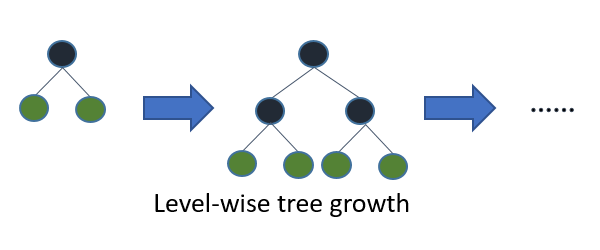
\includegraphics{img/xgboost.png}

}

}

\subcaption{\label{fig-xgboost}\emph{level-wise}}
\end{minipage}%
\newline
\begin{minipage}[t]{\linewidth}

{\centering 

\raisebox{-\height}{

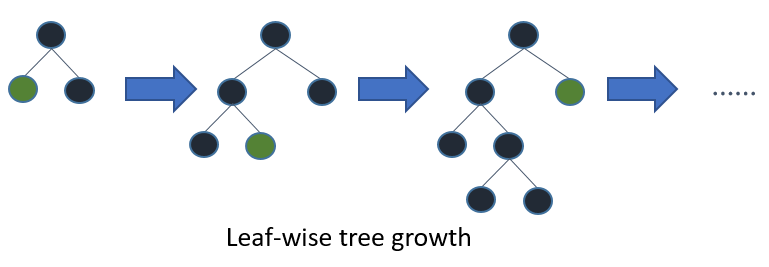
\includegraphics{img/lightgbm.png}

}

}

\subcaption{\label{fig-lightgbm}\emph{leaf-wise}}
\end{minipage}%

\caption{\label{fig-tree-growth}Crescimento de árvores em algoritmos de
\emph{boosting}.}

\end{figure}

\section{Random Forest}\label{random-forest}

Floresta aleatória é um método de aprendizado de máquina que utiliza
conjuntos de árvores de decisão descorrelatadas\footnote{As árvores de
  decisão são descorrelatadas no sentido que, ao contrário os métodos de
  \emph{boosting trees}, a próxima árvore não é construída com base na
  iteração anterior (processo de fortalecimento).} para classificação ou
regressão. O método consiste em treinar várias árvores de decisão em
subconjuntos aleatórios dos dados de treinamento e, então, combinar suas
predições \autocite{hastie_elements_2009}. A aleatoriedade é introduzida
de duas formas: na seleção das observações e na seleção das variáveis
preditoras.

A intuição para seu algoritmo para regressão é simples e a ideia geral
é, para cada árvore de decisão, particionar recursivamente nós de
tamanho \(N\) em dois nós filhos de forma a aumentar a complexidade do
modelo e minimizar a função de custo. Se a próxima partição de um nó
resultar em um ou ambos nós filhos de tamanho menor que um mínimo
estabelecido via hiperparâmetro, a partição é interrompida (Algoritmo
\ref{alg-rf}).

\begin{algorithm}
\caption{Floresta aleatória para regressão}\label{alg-rf}

${T_1, T_2, ..., T_b}$ é uma floresta aleatória de $B$ árvores de decisão. \\
\BlankLine
$i \in \mathbb{N}$ é a quantidade de observações em um nó. \\
\BlankLine
$n_{min} \in \mathbb{N}$ é o número mínimo de observações em um nó. \\
\BlankLine
\For{$b = 1 \to B$}{
  1. Toma uma amostra de tamanho $N$ dos dados de treino. \\
  \While{$i < n_{min}$} {
    a. Seleciona $j$ variáveis aleatoriamente. \\
    b. Escolhe a melhor variável para \textit{split} dentre $j$. \\
    c. Divide o nó em dois nós filhos. \\
    \If{Nenhum dos nós filhos tem $i < n_{min}$} {
      d. Repete os passos a-c para cada nó filho.
    }
  }
}
\BlankLine
2. Produz um conjunto de árvores $\{T_b\}_1^B$.
\BlankLine
3. Realiza a predição para cada árvore $T_b$ em um ponto $x$ e calcula a média das predições:
$$\hat{f}(x) = \frac{1}{B}\sum_{b=1}^B T_b(x)$$

\end{algorithm}

\section{Support Vector Machines}\label{support-vector-machines}

A intuição do métodos de SVMs é mais facilmente compreendida a partir de
uma tarefa de classificação de duas classes. Nesse caso, o objetivo é
encontrar um hiperplano (i.e.~um sub-espaço de dimensão \(n-1\)) que
separe as classes de forma que a margem entre o hiperplano e os pontos
de cada classe seja a maior possível. Então, dado um conjunto de \(N\)
pares de observações e suas respectivas classes,
\(\{(x_i, y_i)\}_{i=1}^N\), em que \(x_i \in \mathbb{R}^p\) e
\(y_i \in \{-1, 1\}\), queremos encontrar o hiperplano definido por

\[
\{x: f(x) = x^T\beta + \beta_0 = 0\}
\]

\noindent sendo \(f(x)\) a distância ortogonal entre \(x\) e o
hiperplano \(f(x) = x^T\beta + \beta_0 = 0\), e \(M\) a margem entre as
classes, definida como a distância ortogonal entre os pontos mais
próximos de cada classe e o hiperplano \autocite{hastie_elements_2009}.
Portanto, o problema de otimização é dado por

\begin{equation}\protect\hypertarget{eq-svm}{}{
\begin{aligned}
& \underset{\beta, \beta_0}{\text{max}}
& & M \\
& \text{sujeito a}
& & y_i(x_i^T\beta + \beta_0) \geq M, \quad i = 1, ..., N
\end{aligned}
}\label{eq-svm}\end{equation}

Quando pode-se encontrar um hiperplano com
\(y_if(x_i) > 0 \quad \forall i\), tem-se o caso da construção de uma
solução única para um hiperplano entre duas classes perfeitamente
separadas pela maior margem possível (Figura~\ref{fig-svm1}).

\begin{figure}

\begin{minipage}[t]{\linewidth}

{\centering 

\raisebox{-\height}{

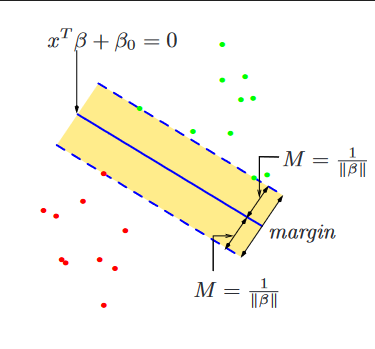
\includegraphics{img/svm1.png}

}

}

\subcaption{\label{fig-svm1}Hiperplano entre duas classes perfeitamente
separáveis.}
\end{minipage}%
\newline
\begin{minipage}[t]{\linewidth}

{\centering 

\raisebox{-\height}{

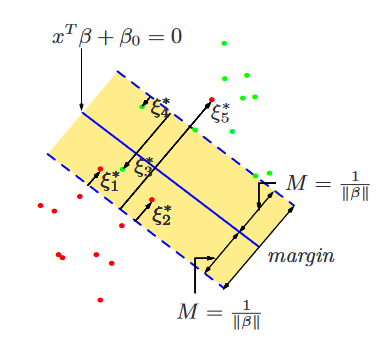
\includegraphics{img/svm2.png}

}

}

\subcaption{\label{fig-svm2}Hiperplano entre duas classes não
separáveis.}
\end{minipage}%

\caption{\label{fig-svm}\emph{Support vector classifiers}. Fonte:
\textcite{hastie_elements_2009}.}

\end{figure}

Entretanto, no mundo real, dificilmente um problema de classificação
será linearmente separável. Paara contornar esse obstáculo, é possível
introduzir variáveis de folga \(\xi_i \geq 0\) para cada observação
(Figura~\ref{fig-svm2}), de forma que a restrição se torne

\begin{equation}\protect\hypertarget{eq-svm2}{}{
y_i(x_i^T\beta + \beta_0) \geq M(1 - \xi_i), \quad i = 1, ..., N
}\label{eq-svm2}\end{equation}

\noindent e a função objetivo se torne

\begin{equation}\protect\hypertarget{eq-svm3}{}{
\min{||\beta||} \quad \text{sujeito a}
\left\{
  \begin{aligned}
    &\quad y_i(x_i^T\beta + \beta_0) \geq M(1 - \xi_i) \quad \forall i, \\
    &\quad \xi_i \geq 0, \sum{\xi_i} \leq \text{constante}
  \end{aligned}
\right\}
}\label{eq-svm3}\end{equation}

Para estender essa ideia para problemas de regressão, é necessário
introduzir uma função de perda \(\epsilon\)-insensível, que penaliza
apenas os erros maiores que \(\epsilon\), de forma que os erros menores
são ignorados durante a otimização, assim como as observações
localizadas no lado correto do hiperplano são ignoradas no problema de
classificação. A função objetivo se torna

\begin{equation}\protect\hypertarget{eq-svm4}{}{
\min{||\beta||} \quad \text{sujeito a}
\left\{
  \begin{aligned}
    &\quad |y_i - x_i^T\beta - \beta_0| \leq \epsilon \quad \forall i, \\
    &\quad \sum{|\beta_j|} \leq \text{constante}
  \end{aligned}
\right\}
}\label{eq-svm4}\end{equation}

% apêndice C
\chapter{CONJUNTO DE HIPERPARÂMETROS} \label{apendice_hiperparametros}

\begin{table}

  \caption{\label{tab:tbl-hip-xgboost}Intervalos de hiperparâmetros para \{xgboost\}}
  \centering
  \begin{tabular}[t]{llll}
  \toprule
  Hiperparâmetro & Descrição & Intervalo & Trafo\\
  \midrule
  \cellcolor{gray!6}{nrounds} & \cellcolor{gray!6}{Número de iterações} & \cellcolor{gray!6}{$[1, 5000]$} & \cellcolor{gray!6}{NULL}\\
  eta & Taxa de aprendizado & $[-4, 0]$ & $10^x$\\
  \cellcolor{gray!6}{max\_depth} & \cellcolor{gray!6}{Profundidade máxima} & \cellcolor{gray!6}{$[1, 20]$} & \cellcolor{gray!6}{NULL}\\
  subsample & Subamostra & $[0.1, 1]$ & NULL\\
  \cellcolor{gray!6}{colsample\_bytree} & \cellcolor{gray!6}{Subamostra de colunas para uma árvore} & \cellcolor{gray!6}{$[0.1, 1]$} & \cellcolor{gray!6}{NULL}\\
  \addlinespace
  colsample\_bylevel & Subamostra de colunas por nível de profundidade & $[0.1, 1]$ & NULL\\
  \cellcolor{gray!6}{lambda} & \cellcolor{gray!6}{Regularização L2} & \cellcolor{gray!6}{$[-10, 10]$} & \cellcolor{gray!6}{$2^x$}\\
  alpha & Regularização L1 & $[-10, 10]$ & $2^x$\\
  \bottomrule
  \end{tabular}
\end{table}

\begin{table}

  \caption{\label{tab:tbl-hip-lightgbm}Intervalos de hiperparâmetros para \{lightgbm\}}
  \centering
  \begin{tabular}[t]{llll}
  \toprule
  Hiperparâmetro & Descrição & Intervalo & Trafo\\
  \midrule
  \cellcolor{gray!6}{num\_iterations} & \cellcolor{gray!6}{Número de iterações} & \cellcolor{gray!6}{$[1, 1000]$} & \cellcolor{gray!6}{NULL}\\
  boosting & Algoritmo de boosting & \{gbdt, dart, goss\} & NULL\\
  \cellcolor{gray!6}{learning\_rate} & \cellcolor{gray!6}{Taxa de aprendizado} & \cellcolor{gray!6}{$[-4, 0]$} & \cellcolor{gray!6}{$10^x$}\\
  num\_leaves & Número de folhas & $[2, 20]$ & NULL\\
  \cellcolor{gray!6}{lambda\_l1} & \cellcolor{gray!6}{Regularização L1} & \cellcolor{gray!6}{$[-12, 12]$} & \cellcolor{gray!6}{$2^x$}\\
  \addlinespace
  lambda\_l2 & Regularização L2 & $[-12, 12]$ & $2^x$\\
  \cellcolor{gray!6}{feature\_fraction} & \cellcolor{gray!6}{Subamostra de colunas} & \cellcolor{gray!6}{$[0.1, 1]$} & \cellcolor{gray!6}{NULL}\\
  bagging\_fraction & Subamostra de linhas & $[0.1, 1]$ & NULL\\
  \cellcolor{gray!6}{bagging\_freq} & \cellcolor{gray!6}{Frequência de amostragem} & \cellcolor{gray!6}{$[1, 10]$} & \cellcolor{gray!6}{NULL}\\
  \bottomrule
  \end{tabular}
\end{table}

\begin{table}

  \caption{\label{tab:tbl-hip-ranger}Intervalos de hiperparâmetros para \{ranger\}}
  \centering
  \resizebox{\linewidth}{!}{
  \begin{tabular}[t]{llll}
  \toprule
  Hiperparâmetro & Descrição & Intervalo & Trafo\\
  \midrule
  \cellcolor{gray!6}{min.node.size} & \cellcolor{gray!6}{Número mínimo de observações em um nó terminal} & \cellcolor{gray!6}{$[1,7]$} & \cellcolor{gray!6}{$2^x$}\\
  mtry & Número de variáveis candidatas para split & $[1,)$ & NULL\\
  \cellcolor{gray!6}{replace} & \cellcolor{gray!6}{Amostragem com reposição} & \cellcolor{gray!6}{\{TRUE, FALSE\}} & \cellcolor{gray!6}{NULL}\\
  sample.fraction & Fração de observações a serem amostradas & $[0.1, 1]$ & NULL\\
  \cellcolor{gray!6}{num.trees} & \cellcolor{gray!6}{Número de árvores} & \cellcolor{gray!6}{$[1, 2000]$} & \cellcolor{gray!6}{NULL}\\
  \bottomrule
  \end{tabular}}
\end{table}

\begin{table}

  \caption{\label{tab:tbl-hip-svm}Intervalos de hiperparâmetros para \{e1071\} (svm)
  }
  \centering
  \begin{tabular}[t]{llll}
  \toprule
  Hiperparâmetro & Descrição & Intervalo & Trafo\\
  \midrule
  \cellcolor{gray!6}{cost} & \cellcolor{gray!6}{Custo de $\xi$} & \cellcolor{gray!6}{$[0, 1]$} & \cellcolor{gray!6}{$2^x$}\\
  kernel & Kernel & \{linear, polynomial, radial, sigmoid\} & NULL\\
  \cellcolor{gray!6}{degree} & \cellcolor{gray!6}{Grau do polinômio} & \cellcolor{gray!6}{$[1, 5]$} & \cellcolor{gray!6}{NULL}\\
  gamma & Influência amostral & $[-12, 12]$ & $2^x$\\
  \cellcolor{gray!6}{type} & \cellcolor{gray!6}{Tipo de SVM} & \cellcolor{gray!6}{\{eps-regression\}} & \cellcolor{gray!6}{NULL}\\
  \bottomrule
  \end{tabular}
\end{table}

\begin{table}

  \caption{\label{tab:tbl-hip-glmnet}Intervalos de hiperparâmetros para \{glmnet\}}
  \centering
  \begin{tabular}[t]{llll}
  \toprule
  Hiperparâmetro & Descrição & Intervalo & Trafo\\
  \midrule
  \cellcolor{gray!6}{alpha} & \cellcolor{gray!6}{Mix entre lasso e ridge} & \cellcolor{gray!6}{$[0, 1]$} & \cellcolor{gray!6}{NULL}\\
  lambda & Regularização & $[-12, 12]$ & $2^x$\\
  \bottomrule
  \end{tabular}
\end{table}

% apendice D
\chapter{RESULTADOS PARA A BASE DE DADOS TOURISM}\label{apendice_tourism}

A base de dados "Tourism" consiste na quantidade trimestral de pernoites
em visitas na Austrália entre 1998 e 2016. A estrutura é hierárquica e
agrupada, composta por 3 níveis hierárquicos --- \emph{State} (Estados),
\emph{Region} (Regiões) e total ---, e agrupado por \emph{Purpose}
(Propósito).

Assim como na base de dados Estban, aqui também não houve uma combinação
de método e estratégia que fosse consistentemente melhor ao longo de
todos os níveis de agregação. Entretanto, uma tendência pode ser
observada em ambas bases de dados, com os métodos de ML se mostrando a
melhor opção para estimação nos níveis ao topo da hierarquia, enquanto
os métodos analíticos se mostram melhor opção para os níveis ao fundo da
hierarquia.

Nessa base de dados, o método SVM na estratégia \emph{rolling forecast}
se mostrou a melhor combinação para os níveis mais agregados, alcançando
93\% de incremento de performance em relação ao MinT, em termos de
RMSSE, ou seja, o MinT teve quase o dobro do erro que o SVM. Já a estratégia \emph{reduced fitted base} teve performance muito baixa, com probelmas de estimação e necessidade de imputação de dados. Além da perda de performance nas medidas de acurácia, a estratégia \emph{reduced fitted base} também teve tempo de processamento muito longos em relação às outras estratégias. Nessa estratégia também foi observada presença de valores negativos para os métodos \emph{elastic net} e SVM, de forma que foram excluídos do \emph{benchmark}.

\hypertarget{tbl-tourism-results-analiticos}{}
\begin{table}
\caption{\label{tbl-tourism-results-analiticos}Resultados Tourism: Acurácia dos métodos analíticos de reconciliação }\tabularnewline

\centering
\begin{tabular}[t]{lrrrr>{}r>{}r}
\toprule
.model & agregado & state & region & purpose & bottom & hierarquia\\
\midrule
\addlinespace[0.3em]
\multicolumn{7}{l}{\textbf{RMSSE}}\\
\cellcolor{gray!10}{\hspace{1em}base} & \cellcolor{gray!10}{1.446} & \cellcolor{gray!10}{1.260} & \cellcolor{gray!10}{1.068} & \cellcolor{gray!10}{1.265} & \cellcolor{gray!10}{0.925} & \cellcolor{gray!10}{0.976}\\
\hspace{1em}bu & 2.580 & 1.634 & 1.113 & 2.004 & 0.925 & 1.011\\
\cellcolor{gray!10}{\hspace{1em}mint} & \cellcolor{gray!10}{1.813} & \cellcolor{gray!10}{1.296} & \cellcolor{gray!10}{0.978} & \cellcolor{gray!10}{1.420} & \textbf{\cellcolor{gray!10}{0.876}} & \textbf{\cellcolor{gray!10}{0.923}}\\
\addlinespace[0.3em]
\multicolumn{7}{l}{\textbf{MASE}}\\
\hspace{1em}base & 1.533 & 1.399 & 1.132 & 1.330 & 0.979 & 1.036\\
\cellcolor{gray!10}{\hspace{1em}bu} & \cellcolor{gray!10}{3.164} & \cellcolor{gray!10}{1.877} & \cellcolor{gray!10}{1.176} & \cellcolor{gray!10}{2.323} & \cellcolor{gray!10}{0.979} & \cellcolor{gray!10}{1.078}\\
\hspace{1em}mint & 2.086 & 1.449 & 1.021 & 1.512 & \textbf{0.937} & \textbf{0.984}\\
\bottomrule
\end{tabular}
\end{table}

\hypertarget{tbl-tourism-results-ml-rolling}{}
\begin{table}
\caption{\label{tbl-tourism-results-ml-rolling}Resultados Tourism: Acurácia dos métodos de ML de reconciliação.
Estratégia rolling forecast. }\tabularnewline

\centering
\begin{tabular}[t]{l>{}r>{}rr>{}rrr}
\toprule
modelo & agregado & State & Region & Purpose & bottom & hierarquia\\
\midrule
\addlinespace[0.3em]
\multicolumn{7}{l}{\textbf{RMSSE}}\\
\cellcolor{gray!10}{\hspace{1em}elastic net} & \cellcolor{gray!10}{1.990} & \cellcolor{gray!10}{1.386} & \cellcolor{gray!10}{1.086} & \cellcolor{gray!10}{1.541} & \cellcolor{gray!10}{0.988} & \cellcolor{gray!10}{1.041}\\
\hspace{1em}lasso & 1.929 & 1.373 & 1.100 & 1.523 & 1.026 & 1.069\\
\cellcolor{gray!10}{\hspace{1em}lightgbm} & \cellcolor{gray!10}{4.330} & \cellcolor{gray!10}{2.762} & \cellcolor{gray!10}{1.651} & \cellcolor{gray!10}{3.456} & \cellcolor{gray!10}{1.141} & \cellcolor{gray!10}{1.354}\\
\hspace{1em}ranger & 2.135 & 1.365 & 1.033 & 1.709 & 0.908 & 0.966\\
\cellcolor{gray!10}{\hspace{1em}ridge} & \underline{\cellcolor{gray!10}{1.256}} & \underline{\cellcolor{gray!10}{1.185}} & \cellcolor{gray!10}{1.013} & \underline{\cellcolor{gray!10}{1.202}} & \cellcolor{gray!10}{0.919} & \cellcolor{gray!10}{0.959}\\
\hspace{1em}svm & \textbf{0.940} & \textbf{1.010} & 1.076 & \textbf{1.011} & 1.100 & 1.097\\
\cellcolor{gray!10}{\hspace{1em}xgb} & \cellcolor{gray!10}{2.340} & \cellcolor{gray!10}{1.451} & \cellcolor{gray!10}{1.114} & \cellcolor{gray!10}{1.892} & \cellcolor{gray!10}{0.964} & \cellcolor{gray!10}{1.031}\\
\addlinespace[0.3em]
\multicolumn{7}{l}{\textbf{MASE}}\\
\hspace{1em}elastic net & 2.360 & 1.572 & 1.145 & 1.653 & 1.058 & 1.115\\
\cellcolor{gray!10}{\hspace{1em}lasso} & \cellcolor{gray!10}{2.264} & \cellcolor{gray!10}{1.557} & \cellcolor{gray!10}{1.168} & \cellcolor{gray!10}{1.593} & \cellcolor{gray!10}{1.110} & \cellcolor{gray!10}{1.155}\\
\hspace{1em}lightgbm & 5.505 & 3.214 & 1.763 & 4.060 & 1.200 & 1.448\\
\cellcolor{gray!10}{\hspace{1em}ranger} & \cellcolor{gray!10}{2.579} & \cellcolor{gray!10}{1.528} & \cellcolor{gray!10}{1.073} & \cellcolor{gray!10}{1.816} & \cellcolor{gray!10}{0.961} & \cellcolor{gray!10}{1.020}\\
\hspace{1em}ridge & \underline{1.343} & \underline{1.309} & 1.058 & \underline{1.192} & 0.981 & 1.020\\
\cellcolor{gray!10}{\hspace{1em}svm} & \textbf{\cellcolor{gray!10}{1.070}} & \textbf{\cellcolor{gray!10}{1.096}} & \cellcolor{gray!10}{1.140} & \textbf{\cellcolor{gray!10}{1.033}} & \cellcolor{gray!10}{1.178} & \cellcolor{gray!10}{1.174}\\
\hspace{1em}xgb & 2.888 & 1.650 & 1.162 & 2.118 & 1.013 & 1.087\\
\bottomrule
\end{tabular}
\end{table}

\hypertarget{tbl-tourism-results-ml-fitted}{}
\begin{table}
\caption{\label{tbl-tourism-results-ml-fitted}Resultados Tourism: Acurácia dos métodos de ML de reconciliação.
Estratégia fitted base. }\tabularnewline

\centering
\begin{tabular}[t]{lr>{}r>{}r>{}rrr}
\toprule
modelo & agregado & State & Region & Purpose & bottom & hierarquia\\
\midrule
\addlinespace[0.3em]
\multicolumn{7}{l}{\textbf{RMSSE}}\\
\cellcolor{gray!10}{\hspace{1em}elastic net} & \cellcolor{gray!10}{2.17} & \cellcolor{gray!10}{1.40} & \cellcolor{gray!10}{1.10} & \cellcolor{gray!10}{1.77} & \cellcolor{gray!10}{0.97} & \cellcolor{gray!10}{1.03}\\
\hspace{1em}lasso & 1.90 & 1.45 & 1.09 & 1.61 & 0.97 & 1.03\\
\cellcolor{gray!10}{\hspace{1em}lightgbm} & \cellcolor{gray!10}{4.33} & \cellcolor{gray!10}{2.76} & \cellcolor{gray!10}{1.65} & \cellcolor{gray!10}{3.46} & \cellcolor{gray!10}{1.14} & \cellcolor{gray!10}{1.35}\\
\hspace{1em}ranger & 2.12 & 1.36 & 1.03 & 1.72 & 0.91 & 0.96\\
\cellcolor{gray!10}{\hspace{1em}ridge} & \cellcolor{gray!10}{1.57} & \underline{\cellcolor{gray!10}{1.16}} & \textbf{\cellcolor{gray!10}{0.97}} & \cellcolor{gray!10}{1.29} & \cellcolor{gray!10}{0.90} & \cellcolor{gray!10}{0.93}\\
\hspace{1em}svm & 1.50 & \underline{1.19} & 1.05 & 1.38 & 1.04 & 1.05\\
\cellcolor{gray!10}{\hspace{1em}xgb} & \cellcolor{gray!10}{2.27} & \cellcolor{gray!10}{1.42} & \cellcolor{gray!10}{1.10} & \cellcolor{gray!10}{1.83} & \cellcolor{gray!10}{0.96} & \cellcolor{gray!10}{1.02}\\
\addlinespace[0.3em]
\multicolumn{7}{l}{\textbf{MASE}}\\
\hspace{1em}elastic net & 2.59 & 1.57 & 1.16 & 1.95 & 1.04 & 1.10\\
\cellcolor{gray!10}{\hspace{1em}lasso} & \cellcolor{gray!10}{2.21} & \cellcolor{gray!10}{1.67} & \cellcolor{gray!10}{1.16} & \cellcolor{gray!10}{1.73} & \cellcolor{gray!10}{1.04} & \cellcolor{gray!10}{1.11}\\
\hspace{1em}lightgbm & 5.50 & 3.21 & 1.76 & 4.06 & 1.20 & 1.45\\
\cellcolor{gray!10}{\hspace{1em}ranger} & \cellcolor{gray!10}{2.54} & \cellcolor{gray!10}{1.54} & \cellcolor{gray!10}{1.07} & \cellcolor{gray!10}{1.84} & \cellcolor{gray!10}{0.97} & \cellcolor{gray!10}{1.02}\\
\hspace{1em}ridge & 1.77 & \underline{1.29} & \textbf{1.01} & \underline{1.31} & 0.96 & 0.99\\
\cellcolor{gray!10}{\hspace{1em}svm} & \cellcolor{gray!10}{1.75} & \underline{\cellcolor{gray!10}{1.30}} & \cellcolor{gray!10}{1.09} & \cellcolor{gray!10}{1.36} & \cellcolor{gray!10}{1.10} & \cellcolor{gray!10}{1.11}\\
\hspace{1em}xgb & 2.79 & 1.62 & 1.15 & 2.04 & 1.01 & 1.08\\
\bottomrule
\end{tabular}
\end{table}

\hypertarget{tbl-tourism-results-ml-refit}{}
\begin{table}
\caption{\label{tbl-tourism-results-ml-refit}Resultados Tourism: Acurácia dos métodos de ML de reconciliação.
Estratégia reduced fitted base. }\tabularnewline

\centering
\begin{tabular}[t]{lrrrrrr}
\toprule
modelo & agregado & State & Region & Purpose & bottom & hierarquia\\
\midrule
\addlinespace[0.3em]
\multicolumn{7}{l}{\textbf{RMSSE}}\\
\cellcolor{gray!10}{\hspace{1em}lightgbm} & \cellcolor{gray!10}{4.33} & \cellcolor{gray!10}{2.76} & \cellcolor{gray!10}{1.65} & \cellcolor{gray!10}{3.46} & \cellcolor{gray!10}{1.14} & \cellcolor{gray!10}{1.35}\\
\hspace{1em}ranger & 2.58 & 1.55 & 1.11 & 2.01 & 0.92 & 1.01\\
\cellcolor{gray!10}{\hspace{1em}xgb} & \cellcolor{gray!10}{3.14} & \cellcolor{gray!10}{1.93} & \cellcolor{gray!10}{1.28} & \cellcolor{gray!10}{2.44} & \cellcolor{gray!10}{1.02} & \cellcolor{gray!10}{1.14}\\
\addlinespace[0.3em]
\multicolumn{7}{l}{\textbf{MASE}}\\
\hspace{1em}lightgbm & 5.50 & 3.21 & 1.76 & 4.06 & 1.20 & 1.45\\
\cellcolor{gray!10}{\hspace{1em}ranger} & \cellcolor{gray!10}{3.18} & \cellcolor{gray!10}{1.76} & \cellcolor{gray!10}{1.17} & \cellcolor{gray!10}{2.24} & \cellcolor{gray!10}{0.98} & \cellcolor{gray!10}{1.07}\\
\hspace{1em}xgb & 3.93 & 2.27 & 1.38 & 2.86 & 1.07 & 1.21\\
\bottomrule
\end{tabular}
\end{table}

\hypertarget{tbl-tourism-tempo-ml}{}
\begin{table}
\caption{\label{tbl-tourism-tempo-ml}Resultados Tourism: Tempo de processamento dos métodos de ML (em horas) }\tabularnewline

\centering
\begin{tabular}[t]{lrrrrrrr}
\toprule
  & xgb & ranger & elastic net & lasso & ridge & svm & lightgbm\\
\midrule
\cellcolor{gray!10}{fitted base} & \cellcolor{gray!10}{15.767} & \cellcolor{gray!10}{3.687} & \cellcolor{gray!10}{1.540} & \cellcolor{gray!10}{1.282} & \cellcolor{gray!10}{1.371} & \cellcolor{gray!10}{1.977} & \cellcolor{gray!10}{3.535}\\
rolling forecast & 12.087 & 2.987 & 0.957 & 0.796 & 1.073 & 2.035 & 3.596\\
\cellcolor{gray!10}{reduced fitted base} & \cellcolor{gray!10}{24.627} & \cellcolor{gray!10}{15.386} & \cellcolor{gray!10}{6.006} & \cellcolor{gray!10}{4.968} & \cellcolor{gray!10}{5.323} & \cellcolor{gray!10}{10.474} & \cellcolor{gray!10}{19.362}\\
\bottomrule
\end{tabular}
\end{table}

\end{apendicesenv}

% anexos 
%\begin{anexosenv}
%\partanexos
%
%
%
%\end{anexosenv}

% índice remissivo 
%\phantompart
%\printindex
